\begin{figure*}[h]

\centering
\begin{minipage}{0.55\textwidth}

\begin{minipage}{0.41\linewidth}
\centering
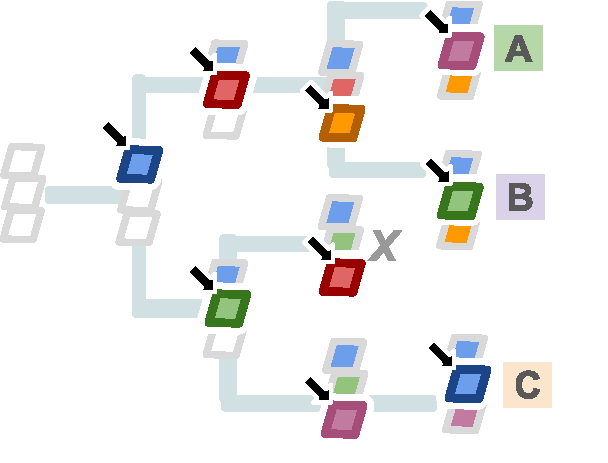
\includegraphics[height=1.1in]{img/hstratschematic-evolve}
\subcaption{evolve}
\label{fig:hstratschematic:evolve}
\end{minipage}%
\vrule
\centering
\begin{minipage}{0.18\linewidth}
~
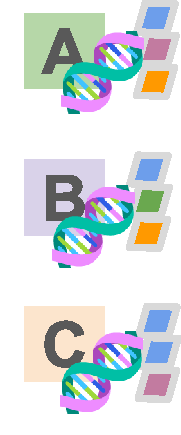
\includegraphics[height=1.1in]{img/hstratschematic-sample}
\subcaption{sample}
\label{fig:hstratschematic:sample}
\end{minipage}%
\vrule
\begin{minipage}{0.41\linewidth}
\centering
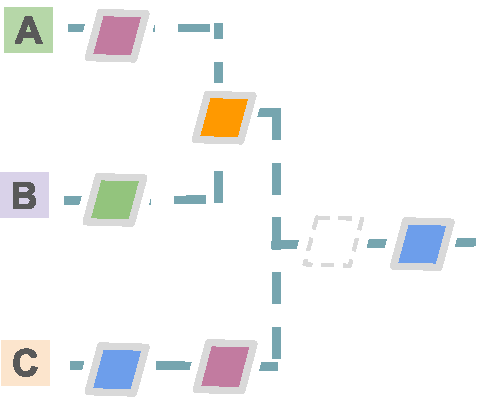
\includegraphics[height=1.1in]{img/hstratschematic-reconstruct}
\subcaption{reconstruct}
\label{fig:hstratschematic:reconstruct}
\end{minipage}
\end{minipage}%
~~
\begin{minipage}{0.43\textwidth}
\caption{%
\textbf{Overview of hereditary stratigraphy.}
\small
At runtime, genomes are annotated with randomly-generated heritable markers (panel \ref{fig:hstratschematic:evolve}).
To maintain fixed-memory footprint, some markers are overwritten.
Genomes of interest are sampled at runtime and from end state (panel \ref{fig:hstratschematic:sample}).
Decoded genome markers enable estimation of evolutionary relatedness (panel \ref{fig:hstratschematic:reconstruct}), subject to error from marker-value collisions and discarded markers.
Adapted from \citet{singhvi2025scalable}.
}
\label{fig:hstratschematic}
\end{minipage}
\end{figure*}
